\section{Delefiltre}
\label{Delefiltre}
Som vist i \fxnote{Hvor er det beskrevet? i Saras ISO-databehandling}, er der tre nævneværdige segmenter på kurven. Hvert segment skal behandles forskelligt, hvorfor der er behov for først at dele signalet ind i tre delsignaler; et fra 0-1000hz, et fra 1000-8000hz og et fra 8000hz og opefter. Ifølge \textcite{PDF:Elektroakustik}, ligger frekvenslejet for grundtonen for et typisk musikinstrument mellem  40Hz og 1000Hz, med overtonefrekvenser langt over den menneskelige hørelse. Dertil kommer de lyde som kan produceres fra en computer eller synthesizer.\\\textcite{STD:ISO226} Afdækker kun den menneskelige hørelse inden for frekvenslejet 20Hz to 12500Hz, men frekvenserne fra 20Hz og nedefter og fra 12kHz og opefter kan med fordel medtages i henholdavis et lav- og højpass filter, da det udgør et simplere filter, og samtidig undgår uforudsete konsekvenser for lyden ved fraskæring, omend, i nogle tilfælde, uden for det hørbare område.\\
Et analogt delefilter bør i teorien kunne have et uendeligt antal band-pass filtre, men er begrænset af hvor præcist et udsnit der kan laves. Man kan eksempelvis ikke lave et filter som udelukkende lukker 1kHz-toner igennem, fordi der er en unøjagtighed nær cutoff-frekvensen, som kaldes for et overgangsbånd, som kan ses på \autoref{fig:OvergangsbaandIllustration}.
%
\begin{figure}[H]
	\centering
	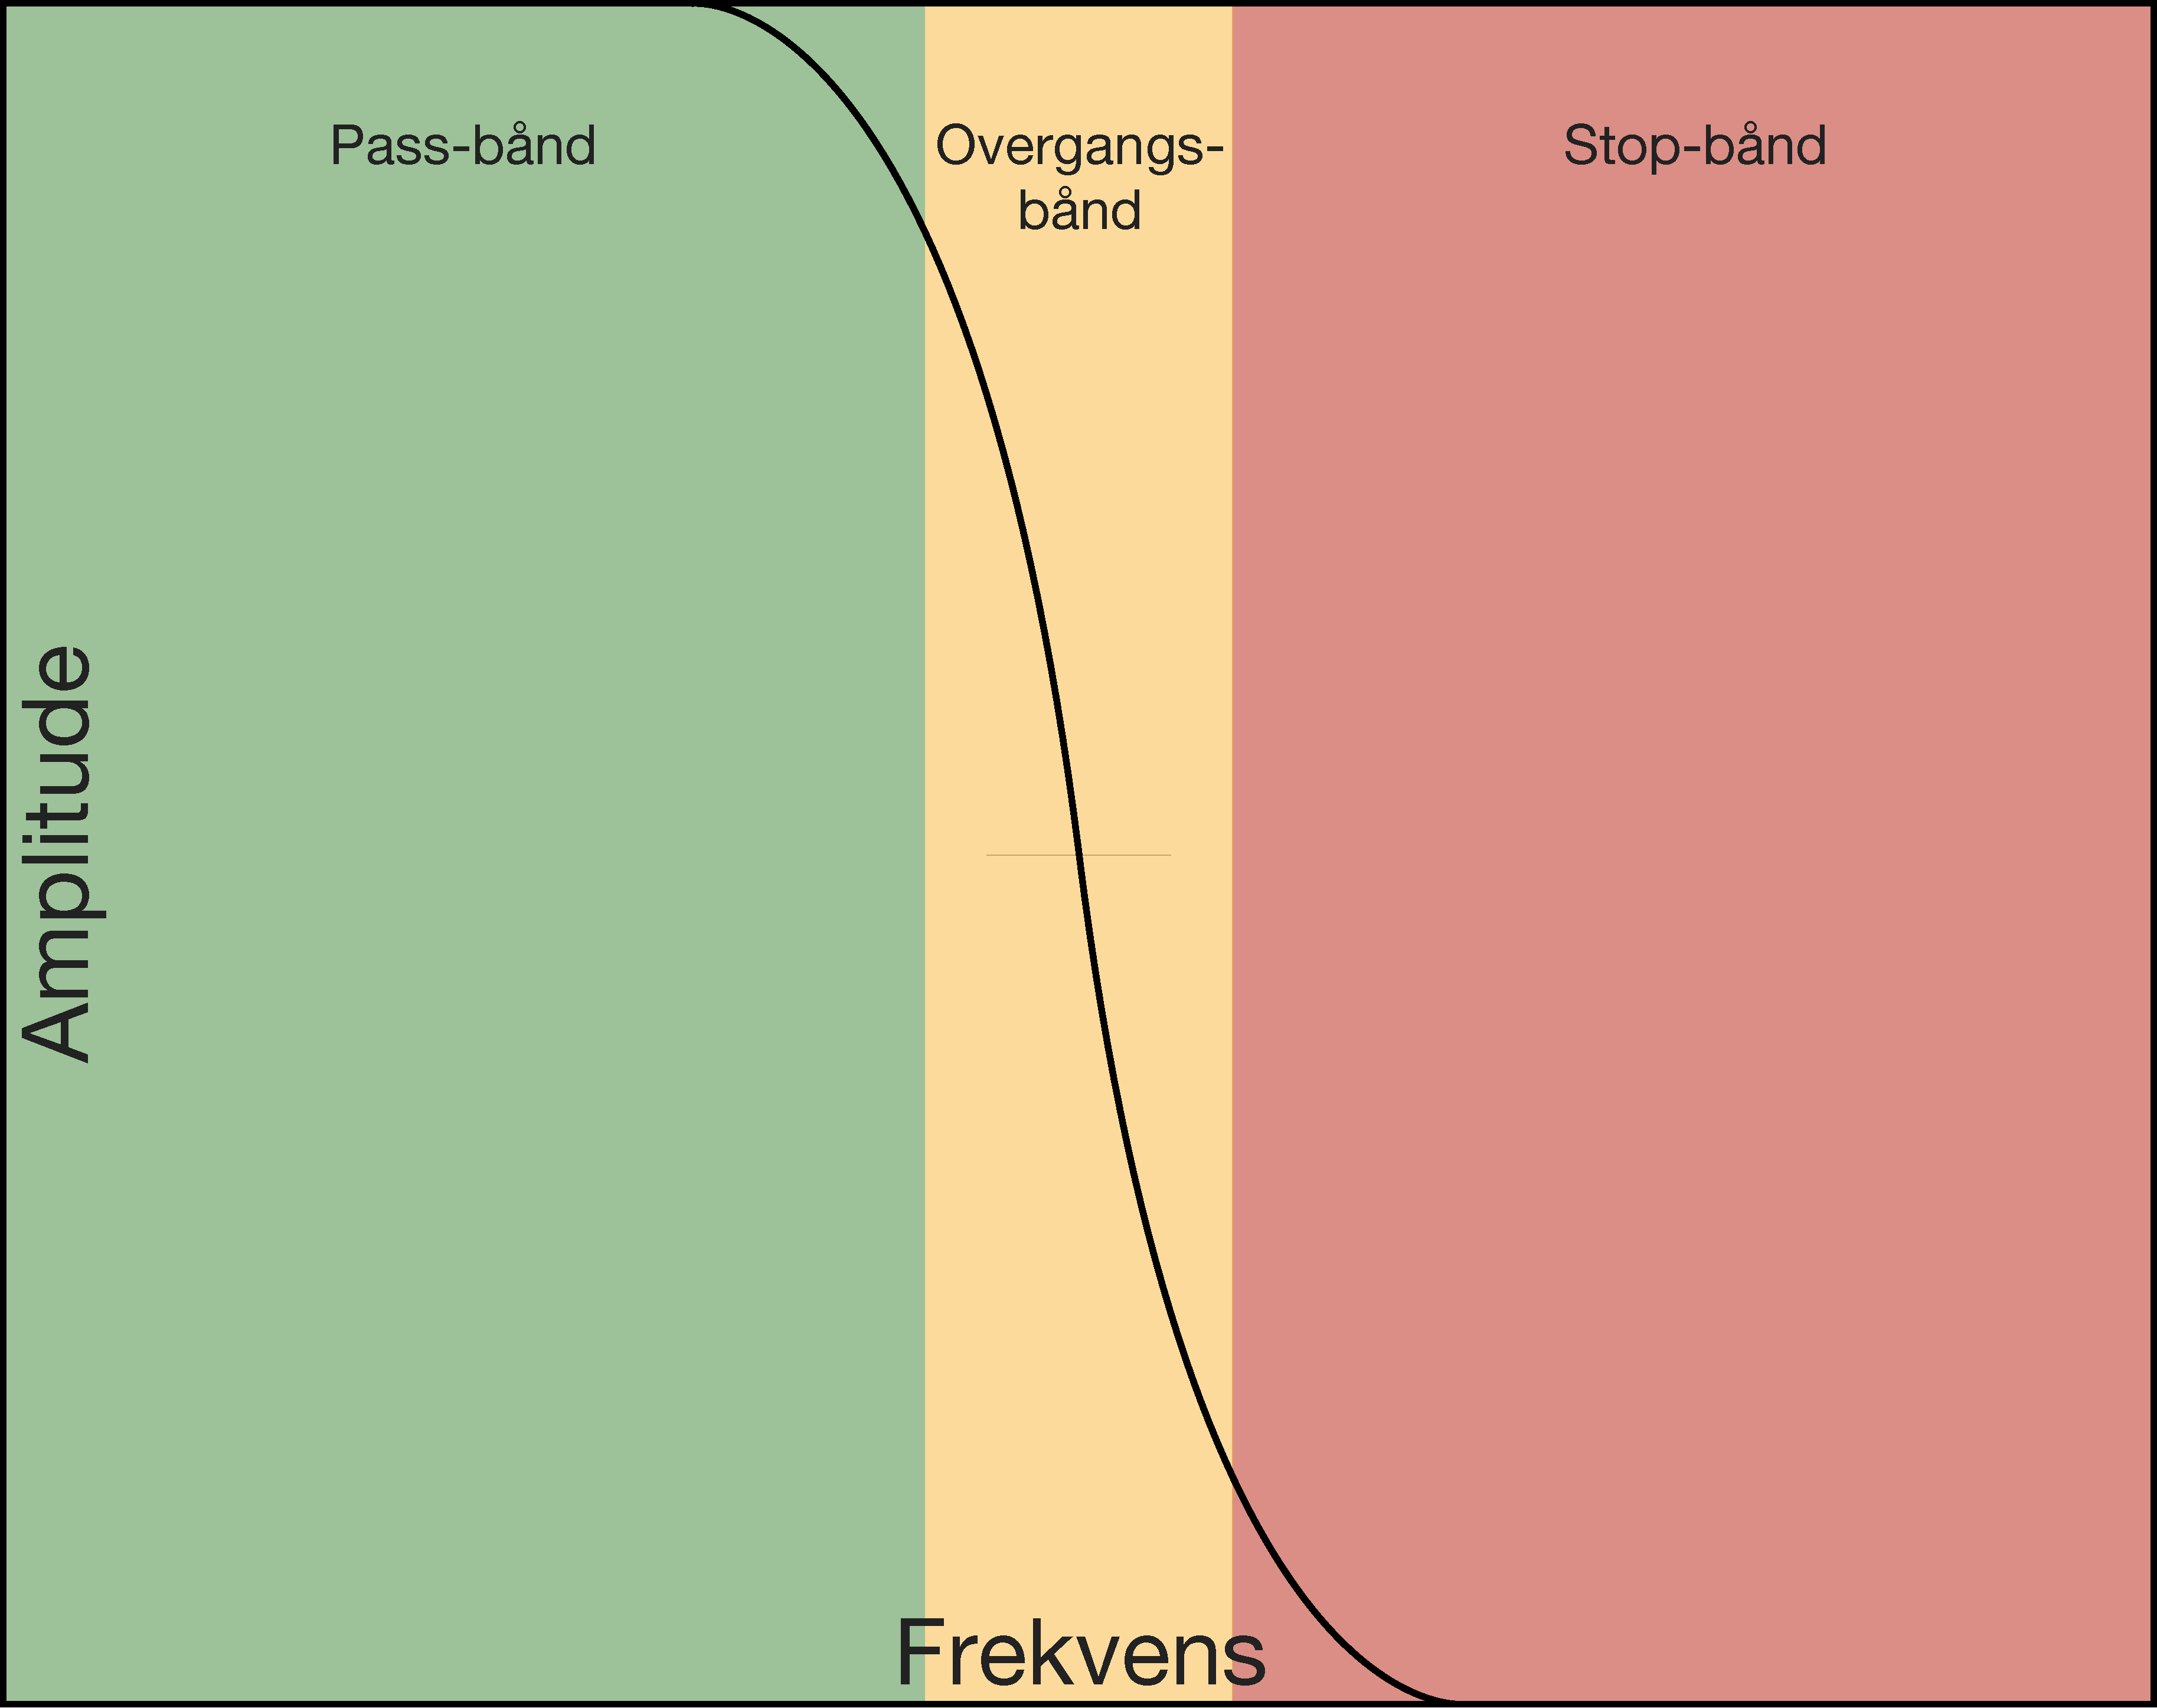
\includegraphics[resolution=300,width=\textwidth/2]{Introduktion/OvergangsbaandIllustration}	
	\caption{Illustration af et typisk overgangsbånd for et low-pass filter. Den grønne firkant er hvad et ideelt filter ville lade passere, men i virkeligheden er det alt under kurven, som medtages. Den gule firkant er således overgangsbåndet, altså et biprodukt af filtret,}
	\label{fig:OvergangsbaandIllustration}
\end{figure}
\noindent
%
Overgangsbåndet er en bivirkning ved alle analoge filtre, men kan minimeres ved at øge ordenen af filteret. Det har dog andre ulemper, som vil blive diskuteret senere.\\
%
%
%
\subsection{Aktive- og passive filtre}
\label{Aktive- og passive filtre}
Filtre kan være enten passive eller aktive, hver med sine egenskaber. Hvilken filtertype man vælger, afhænger af hvilke egenskaber man ønsker, såvel som krav til pris og fysisk størrelse.\\
Passive filtre har den fordel at de kan operere uden tilført strøm, som navnet angiver. De benytter kun passive komponenter som modstande, kondensatorer og spoler og virker bedst ved frekvenser mellem 100Hz og 300MHz \parencite{BOOK:PracticalElectronicsforInventors}. Dets lavere frekvensområde, dets større kapacitans og induktans, hvilket kræver fysisk større komponenter, deraf den nedre grænse. Ved høje frekvenser vil komponenterne interferere med hinanden, deraf den øvre grænse.\\
Aktive filtre, modsat passive, kræver tilført strøm, og benytter en operationsforstærker (OpAmp), sammen med modstande og kondensatorer. De kan håndtere meget lave frekvenser og kan øge spændingen på output, hvis ønsket. De er ofte nemmere at konstruere end passive filtre, og kan laves uden brug for store komponenter. De virker bedst ved frekvenser under 100kHz, som konsekvens af operationsforstærkerens båndbredde og slew-rate \fxnote{Hvad hedder slew rate på dansk?}.\\
Eftersom at mennekser kan høre lyde mellem ca. 20Hz og 20kHz, er et aktivt delefilter at foretrække, da det er bedre egnet end passive filtre, i dette frekvensområde. Af samme årsag vil resten af denne rapport beskæftige sig med disse.
%
%
%
\subsection{Lavpasfiltre}
\label{Lavpasfiltre}
Et lavpasfilter er et filter der, som navnet antyder, lader lave frekvenser passere igennem, men blokerer for høje. På \autoref{fig:ActiveLowPass} ses et aktivt lavpasfilter. At det er aktivt, betyder blot at der er tilkoblet en operationsforstærker efter filtret.
%
\begin{figure}[H]
	\centering
	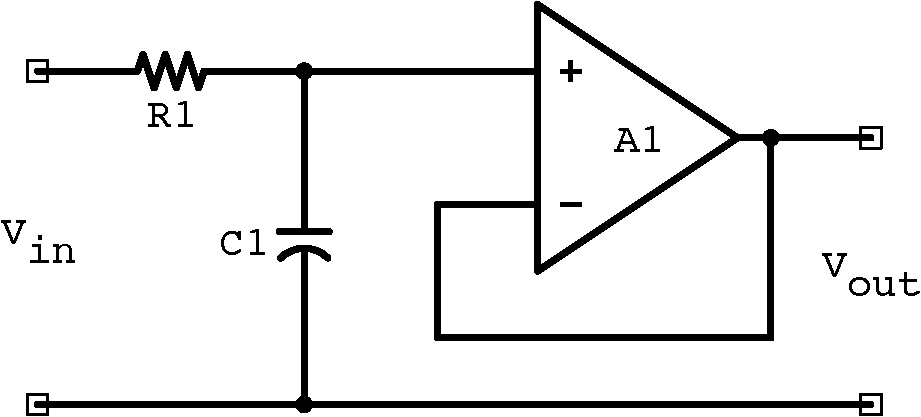
\includegraphics[resolution=300,scale=0.5]{Figure/Introduktion/ActiveLowPass.pdf}
	\caption{Aktivt Lavpasfilter}
	\label{fig:ActiveLowPass}
\end{figure}
\noindent
%
Et lavpasfilter virker ved at kondensatoren, ved høje frekvenser, sænker sin impedans og således lader højre frekvenser gå til jord i stedet for at passere. Modstanden har stor impedans ved høje frekvenser, men lader lave frekvenser passere. Formlen for $V_{out}$ for et passivt filter er:
%
\begin{equation} \label{eq:LowPass_Vout}
	V_{out}=\frac{Z_c}{Z_c+R}*V_{in}
\end{equation}
%
Men det som er mest interessant inden for elektronik, er er \textit{forholdet} mellem $V_{out}$ og $V_{in}$, som kan udtrykkes således:
\begin{equation} \label{eq:LowPass_VOutVin}
	 \left\lvert\frac{V_{out}}{V_{in}}\right\rvert=\frac{1}{\sqrt{1+(\omega RC)^2}}
\end{equation}
\fxnote{Forklar hvad de forskellige ting er i formlerne}
%
Et aktivt filter er blot et passivt filter efterfulgt af en operationsforstærker. I opkoblingen fra \autoref{fig:ActiveLowPass} er der ingen forstærkning af inputsignalet, eftersom tilbagekoblingen går urørt fra $V_{out+}$ til operationsforstærkerens $V_{in-}$. En sådan tilbagekobling kan have fordele, selvom der ikke sker nogen forstærkning. Operationsforstærkerens høje inputimpedans forhindrer overdrevet belastning af filterets output og dens lave outputimpedans sørger for at filtrets afskæringsfrekvens ikke påvirkes af eventuelle ændringer af den efterfølgende impedans. Selvom filteret fra \autoref{fig:Aktivt Lavpasfilter} ikke giver nogen spændingsforstærkelse over 1, giver det en meget høj effekt, grundet at inputimpedansen er langt højere end outputimpedansen. Med andre ord giver det god stabilitet til filteret, men giver ikke nogen spændingsforstærkning. Et kredsløb med forstærkning, kan ses på \autoref{fig:ActiveLowPassGain}.
%
\begin{figure}[H]
	\centering
	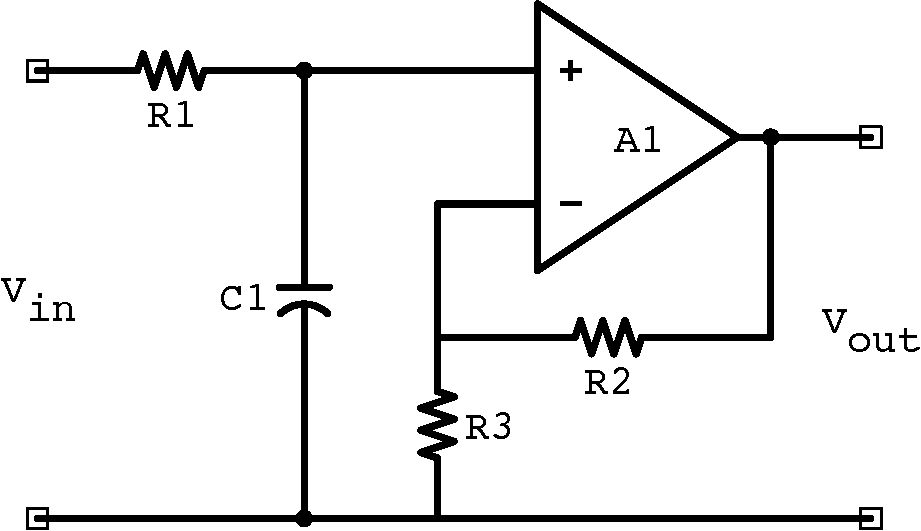
\includegraphics[resolution=300,scale=0.5]{Figure/Introduktion/ActiveLowPassGain.pdf}
	\caption{Aktivt lavpasfilter med forstærkning}
	\label{fig:ActiveLowPassGain}
\end{figure}
\noindent
%
Forholdet mellem modstandene R1 og R2 dikterer $DC$-forstærkningen, og følger, for en ikke-inverterende operationsforstærker, formlen:
%
\begin{equation} \label{eq:LowPassDCGain}
	DC_{gain}=\left(1+\frac{R_2}{R_1}\right)
\end{equation}
%
Sammenholdt med filteret, følger den frekvensafhængige forstærkning af et lavpasfilter således formlen:
%
\begin{equation} \label{LowPassFqVGain}
  V_{gain}=\frac{V_{out}}{V_{in}}=\frac{A_F}{\sqrt{1+\left(\frac{f}{f_c}\right)^2}}
\end{equation}
Hvor:\\
$A_F$ = Forstærkningsfaktoren for operationsforstærkeren, $DC_{gain}$\\
$f$ = Frekvensen af inputsignalet, i Hz\\
$f_c$ = Afskæringsfrekvensen for filteret, i Hz\\
Filteret har konstant forstærkning, $A_F$, fra 0Hz til lidt før afsksæringsfrekvensen $f_c$, hvorefter amplituden falder med en konstant rate på 20dB pr. dekade. Forløbet kan ses på \autoref{fig:FrequencyResponseCurve}.
%
\begin{figure}[H]
	\centering
	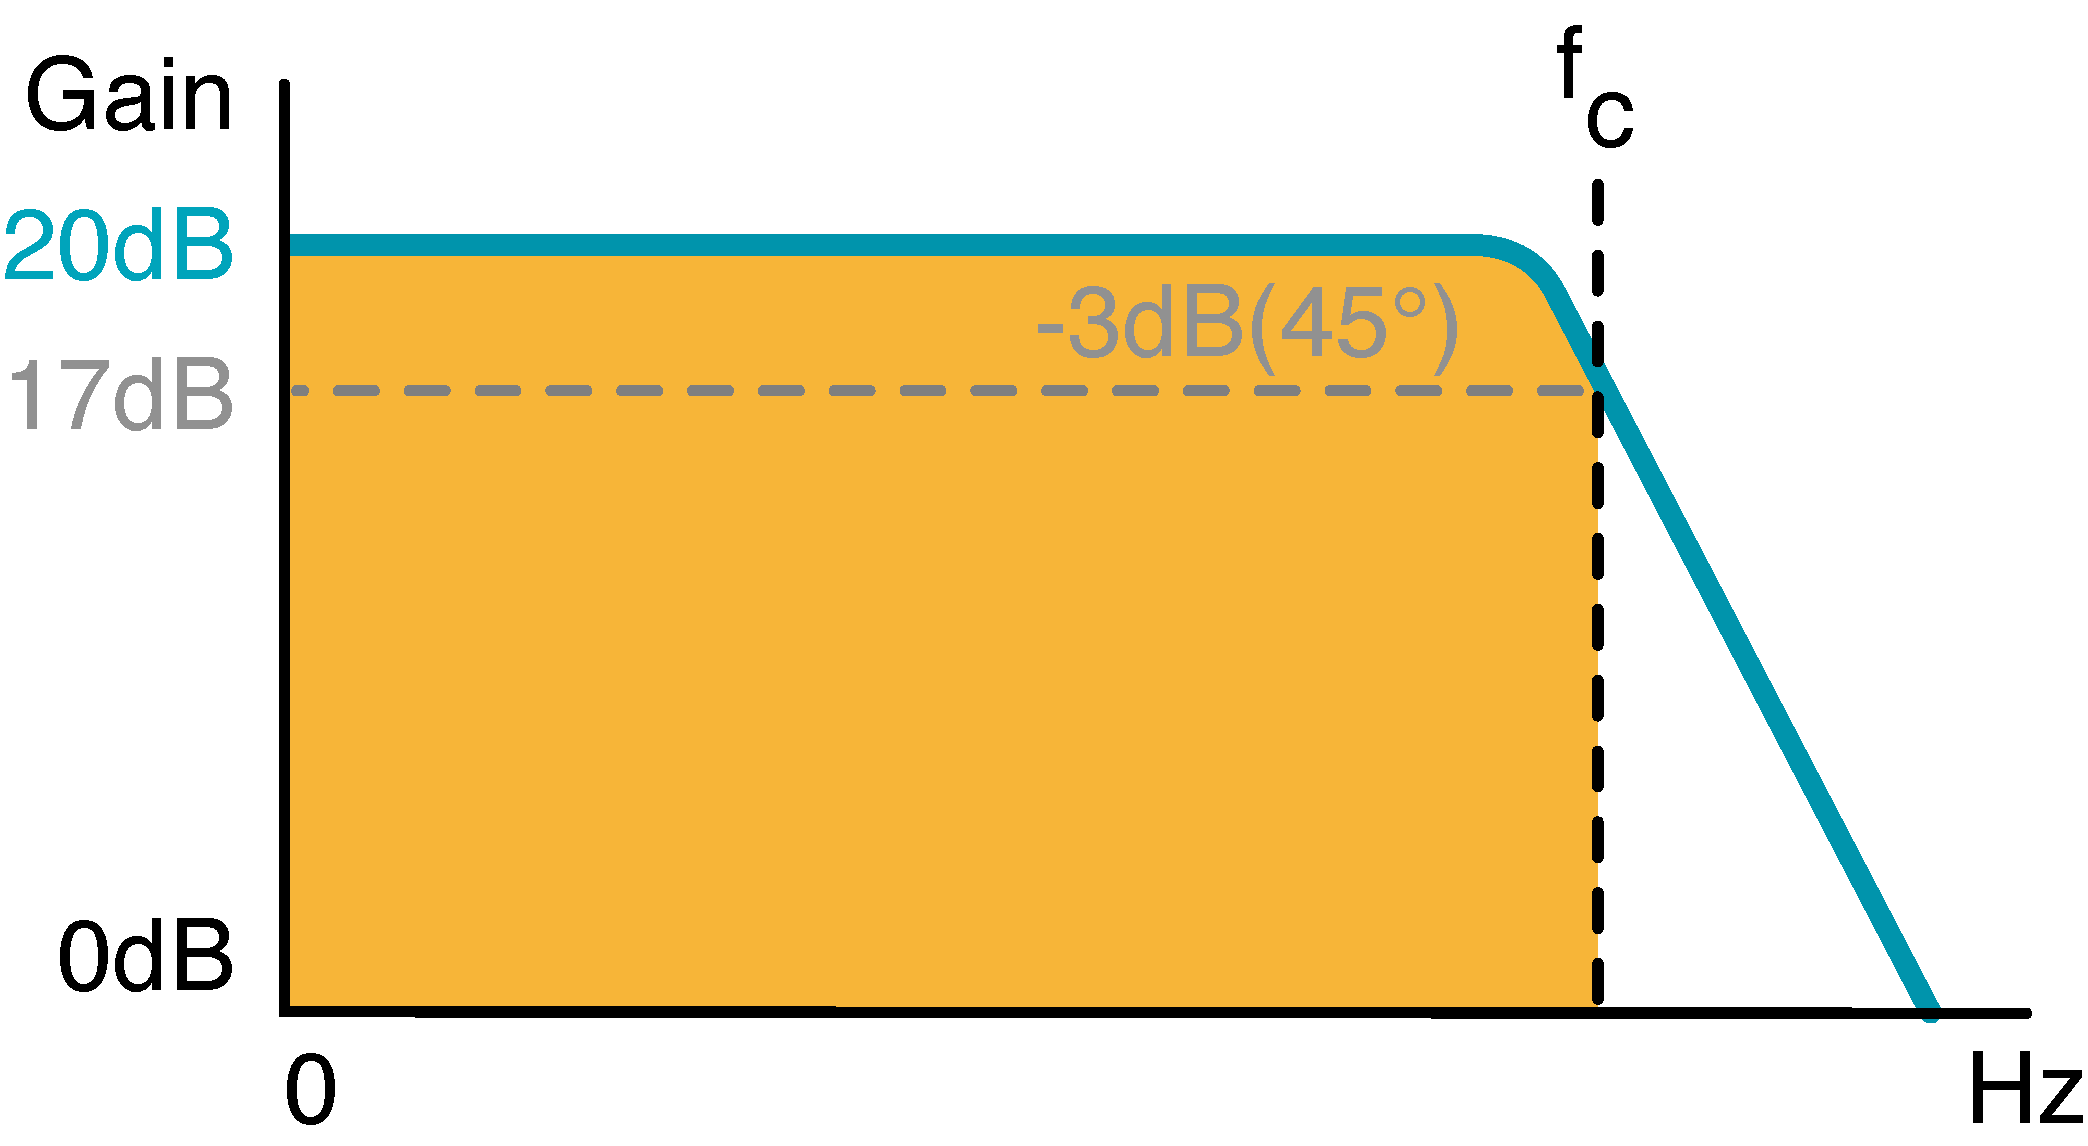
\includegraphics[resolution=300,width=\textwidth/2]{Introduktion/FrequencyResponseCurve}
	\caption{Frekvensresponskurve for et lavpasfilter. Den orange del, er det frekvensområde som medtages i}
	\label{fig:FrequencyResponseCurve}
\end{figure}
\noindent
X\fxnote{skriv figurtekst}
%
%
%
\subsection{Højpasfiltre}
\label{Hoejpasfiltre}
Et højpasfilter er det modsatte af et lavpasfilter, forstået på den måde at det kun lader høje frekvenser passere. Et aktivt lavpasfilter kan ses på....
%
%
%
\subsection{Båndpasfiltre}
\label{Baandpasfiltre}

%Et 
%
%For at lave et delefilter med tre frekvensbånd sammensættes blot et low-pass, band-pass og high-pass filter.
%
